\documentclass[sigconf]{acmart}
\usepackage{booktabs} % For formal tables
\usepackage{graphicx}
\graphicspath{ {images/} }






% Copyright
%\setcopyright{none}
%\setcopyright{acmcopyright}
%\setcopyright{acmlicensed}
\setcopyright{rightsretained}
%\setcopyright{usgov}
%\setcopyright{usgovmixed}
%\setcopyright{cagov}
%\setcopyright{cagovmixed}


% DOI
\acmDOI{10.475/123_4}

% ISBN
\acmISBN{123-4567-24-567/08/06}

%Conference
\acmConference[WOODSTOCK'97]{ACM Woodstock conference}{July 1997}{El
  Paso, Texas USA} 
\acmYear{1997}
\copyrightyear{2016}

\acmPrice{15.00}


\begin{document}
\title{Cryptdump, a data deduplication technique for cryptedb backup}
\titlenote{Produces the permission block, and
  copyright information}
\subtitle{Extended Abstract}
\subtitlenote{The full version of the author's guide is available as
  \texttt{acmart.pdf} document}



\author{Lars Th{\o}rv{\"a}ld}
\authornote{This author is the
  one who did all the really hard work.}
\affiliation{%
  \institution{The Th{\o}rv{\"a}ld Group}
  \streetaddress{1 Th{\o}rv{\"a}ld Circle}
  \city{Hekla} 
  \country{Iceland}}
\email{larst@affiliation.org}

\author{Lawrence P. Leipuner}
\affiliation{
  \institution{Brookhaven Laboratories}
  \streetaddress{P.O. Box 5000}}
\email{lleipuner@researchlabs.org}

\author{Sean Fogarty}
\affiliation{%
  \institution{NASA Ames Research Center}
  \city{Moffett Field}
  \state{California} 
  \postcode{94035}}
\email{fogartys@amesres.org}


% The default list of authors is too long for headers}
\renewcommand{\shortauthors}{B. Trovato et al.}


\begin{abstract}
Security plays a vital role when people deploy services in the cloud,so encryption is ofthen used. Computing over encrypted data has prove useful in such situation. Cryptdb[1] is such kind of system. To support more operation on encrypted data, Cryptdb uses the multi-onion design, which produce significant storage overhead when we need to backup the data. Traditional data deduplication technique do not work well on encrypted data. In this paper, we present the chanllenges we meet when we need to backup data using popular data backup tools, and we propose a new backup method with the help of metadata and implement a new tool Cryptdump for cryptedb. Experiments show that our method can  significantly reduce the storage size with little overhead. Our deduplication method can also be used together with traditional data deduplication methods to further reduce the storage size.


\end{abstract}


%
% The code below should be generated by the tool at
% http://dl.acm.org/ccs.cfm
% Please copy and paste the code instead of the example below. 
%
\begin{CCSXML}
<ccs2012>
 <concept>
  <concept_id>10010520.10010553.10010562</concept_id>
  <concept_desc>Computer systems organization~Embedded systems</concept_desc>
  <concept_significance>500</concept_significance>
 </concept>
 <concept>
  <concept_id>10010520.10010575.10010755</concept_id>
  <concept_desc>Computer systems organization~Redundancy</concept_desc>
  <concept_significance>300</concept_significance>
 </concept>
 <concept>
  <concept_id>10010520.10010553.10010554</concept_id>
  <concept_desc>Computer systems organization~Robotics</concept_desc>
  <concept_significance>100</concept_significance>
 </concept>
 <concept>
  <concept_id>10003033.10003083.10003095</concept_id>
  <concept_desc>Networks~Network reliability</concept_desc>
  <concept_significance>100</concept_significance>
 </concept>
</ccs2012>  
\end{CCSXML}


\ccsdesc[500]{Computer systems organization~Embedded systems}
\ccsdesc[300]{Computer systems organization~Redundancy}
\ccsdesc{Computer systems organization~Robotics}
\ccsdesc[100]{Networks~Network reliability}


\keywords{ACM proceedings, \LaTeX, text tagging}


\maketitle

\section{Introduction}

With the development of cloud computing, more services are deployed in the cloud. Security is the first issue to taken into consideration when people store their data in the cloud. Encryption is an important technique to ensure data security. However, for a database system, when data is encrypted, it could be hard for people to perform operations on those data. Fortunately, with the help of certain encryption schemes, computing over encrypted data is possible. Cryptedb[1], which was proposed in sosp'11, is such kind of system. Similarity system has been implemented by many companies like google,SAP,Microsoft,and some Startups[2][15].


The idea of computing over encrypted data came from homomphic encryption. Fully Homomorphic enctyption is too expensive[9], however, to support common database operation, fully homomorphic is not the only way. The main idea of Cryptdb is to use the characteristics of several encryption schemes to support different operations on columns in a relational table.  Since each encryption scheme can only support one operation, to allow multiple operations, each column in the table is duplicated many times according to how many operations each column need to support, and different encryption schemes are applied to each copy. Such data layout allows computing over encrypted data, but incur huge storage overhead at the same time. According to the author[1], experiments with TPC-C showed an increase of 3.76 times of storage size.

Another import issue of a cloud database system is data intergrety. The system may suffer from disk failures or system crash, so database backup is needed for such systems.

This storage overhead is inevitable when we want to support different operations. However, for a data backup, this duplication is unnecessary since we do not perform operations on the backup.

To reduce storage overhead in backup, data deduplication techniques are ofthen used. In fact, data deduplication has become a standard component for backup systems[10]. However, for cryptdb, traditional deduplication methods are limited since it could be hard to deduplicate encrypted data, and those methods are unaware of the relations between encrypted data. There are research about deduplicating encrypted data, but they focus on user files in the cloud instead of database systems. 

Cryptedb records how the original tables are encrypted and how the columns are replicated. We call those data metadata in this paper. It stores metadata on the proxy. If we introduce this kind of extra information, data deduplication for backup system can be more efficient. And also, the onion layout of fields allow us to make tradeoff between storage size, recover time, and data security.


In this paper, we raise the question that how can we reduce the the overhead of storage with the help of metadata, and that how to use the information to make proper tradeoff. We should consider storage size, security and the time consumed for data recovery. In our work, we propose a new data deduplication method for Cryptdb, which utilizes metadata information to help find duplicates in encrypted data. We implemented a tool called Cryptdbdump and did experiments with TPC-C-MySQL in the newest version of Cryptdb.


To realise this, we need to address three main challenges:

1) How to parse the metadata of Cryptdb

2) How  does the time and space overhead change as the onions and layers change

3) How to choose the right onion and layer to make optimal backup


To tackle those problems, we need to

1) analyse the structure of metadata in Cryptdb and find duplicates

2) do analysis on different onions and layers of encryption scheme and provide statiscis

3) design a strategy for data backup with the help of metadata and the costs information 

To summarize, we make the following contributions.

1) A full analysis of the cost of each layer and onion in Cryptdb

2) A new data deduplication method for Cryptdb that utilizes metadata information 

3) A strategy for choosing the right portion of data for backup, which taken storage size, 

4) An implementation of data backup tool called Cryptedbdump 

To our knowledge, we are the first to propose a deduplication method for Cryptdb with the help of metadata to reduce storage overhead, and our high level deduplication method can be used together with traditional deduplication techniques like block level comparision[12].

The rest of this paper is structured as follows. In section 2, we introduce the structure of cryptdb and the structure of encryption metadata in the newest version of Cryptdb. Then, we introduction the characteristics of the encryption schemes use in Cryptdb in section 3. And in section 4, we introduce popular data backup and deduplication methods. In section 5, we introduce our design details and results of experiments. In section 6 we introduce related work. And Section 7 concludes the paper.
\\ \\ \\ 





\section{Introduction to Cryptdb}

This section introduces the structure of Cryptdb to show how data is duplicated. This introduction is based on the original paper and the newest verion of Cryptdb implementation. We would like to introduce the following content.

1. structure of client, proxy, and MySQL server\\
2. structure of metadata storage\\
3. datalayout \\

This section will give you insight on how we find duplicates in Cryptdb, and important issues to consider when designing a backup system.

\subsection{The client,server, proxy structure}

In the cryptdb system design, there are three identities, client, server, and proxy. The Client is the webserver, and the server has MySQL installed. The client communicate with the proxy instead of with the server. The MySQL server is not trusted while the Proxy is trusted. When the client receive DDL queries, it will stored related metadata to describe the encryption schema of each table. For both DML and DDL queries, the proxy perform query rewrite to encrypt the query and send encrypted query to MySQL server. The results are sent to the proxy first for decryption, and then plain text will be sent to client.


\subsection{metadata layout and structure}

This section talks about metadata layout and the conresponding encryption scheme. Those scheme will impact how we make choices when we bakcup data. The metadata form a hirechy from the database level to the encryption layer level. It has a structure of a tree.


\begin{figure}[tb]
\centering
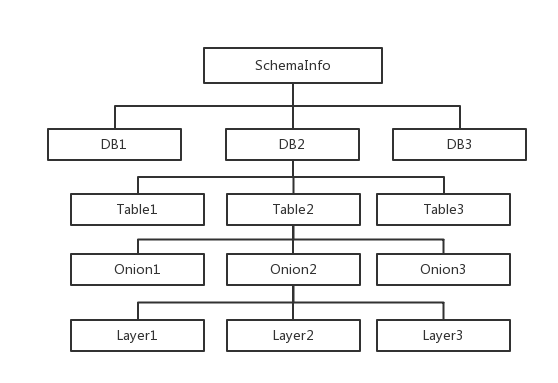
\includegraphics[width=8cm]{onionmeta.png}
\caption{Onionmeta layout}
\label{fig:stack}
\end{figure}

Every node in the tree is storaed as a record with a unique id in a relational table. The relation among nodes and the content of a node is also stored in the same table. Each onion represents an encryption scheme, which has many layers. This tree structure can be stored in a simple relational table, 

CREATE TABLE MetaObject(id bigint(20) unsigned auto\_increment, parent\_id bigint(20),serial\_key varbinary(500),serial\_object varbinary(500));  


So the metadata of databases, tables, fields, onions, layers are all serialized and stored in the proxy. Since the amount of data is related only to the number tables and the number of fields in those tables, the storage size is small. Also, metadata is needed for decryption and data recovery, so we use physical backup and do not deduplicate the metadata. Metadata is in the form is plaintext, so traditional deduplication techinques can work properly.



\section{Encryption schemes}


\subsection{data layers for string type}

For string type, the newest version of cryptdb only support two onions: DET and OPE. Search was removed. Also, since the onion search has only one layer and it's quit easy to do analysis, we focus on the other two layers
in this section. For onion DET, the DET layers uses 128bits AEC-CMC encryption, which is a simple wrapper function of AES-CBC. AES-CBC will pad the plaintext if the size of plaintext can not be divided by the block size. For simplicity, in the current inplementation, if the input can be diveded by the block size, the size of the datatype is expanded by one block size. So, as we add more layers to the onion, the size of the datatype keeps increasing. 

For OPE-str, the data type will be transformed to 64 bits integer. Therefore, the characteristic of OPE-str is constrained to 64bits. The for the RND layer, blowfish will be used since the data type is transformed to integer. OPE is used only for comparing and sinced it loses information, we can not decrypt ope-str. So this onion is not suitable for backup. 

Figure 3.2 provides illustration of the onions. 



\begin{figure}[tb]
\centering
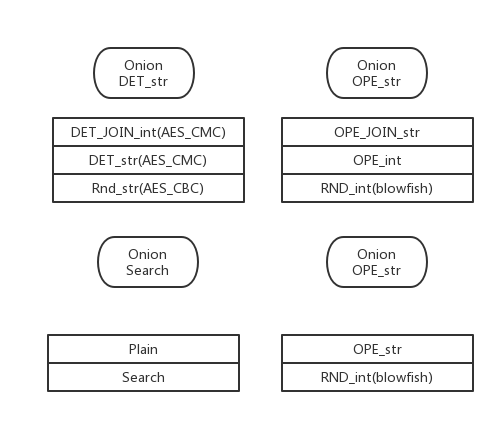
\includegraphics[width=8cm]{Onion_str.png}
\caption{Onion encryption layers for string type}
\label{fig:stack}
\end{figure}




\subsection{data layers for integer}

For integer type, cryptdb create three onion: DET, OPE, and HOM. Figure 3.1 shows the layout of the onions. Hom expand any type of integer to 2048 bits binarychar. For DET and OPE, the type conversion is more complex. DET layer uses blowfish encryption, which requires 64bits integer. RND for integer also uses blowfish encryption. So for DET onion, any integer will be at most expanded to 64 bits long. For onion OPE, the first layer requires that the size of cipher text is twice the size of plaintext. If the size of ciphertext is larger than 64bits thus unable to fit into an integer type, varbinary is used instead. 



\subsection{data layout and structure}

In this section, we talk about the onion layout and How an original table is expanded whith a specific onionlayout. Since the only two data type supported for encryption, we will use and imginery table with those two data types. 








\begin{figure}[tb]
\centering
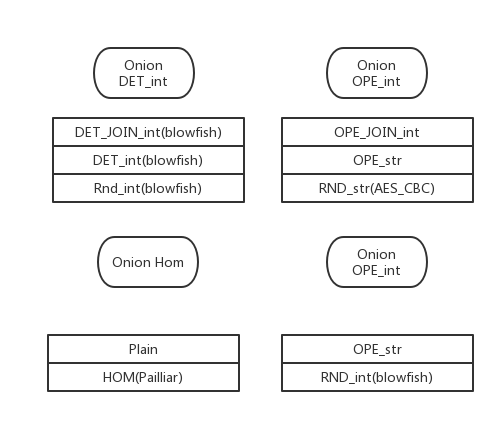
\includegraphics[width=8cm]{Onion_int.png}
\caption{Onion encryption layers for integer type}
\label{fig:stack}
\end{figure}


\section{database backup methods and deduplication}

Data backup is an important functionality of database systems. All the popular database systems have backup methods. Based on how the backup is stored, we can can have two categorities of backup methods: logical backup and physical backup. Backup tools focus on low storage overhead and fast recovery. Since we do experiment with MySQL, this section focus on backup methods for MySQL. 


\subsection{logical backup}
Logical backup save information in the form of SQL queries[14]. For Logical backup, it's easy to control the backup granularity, and it's highly portable since the backup is in text format. MySQLdump and MySQLdumper are examples of Logical backup tools. 



\subsection{physical backup}

Physical bakcup consists of raw copies of directories and files that store the database contents[14].

xbackup. xxxxxx. With the help of metadata and analysis of the file format, we should be able to deduplicate with physical backup. we leave it to future work. 



\section{our design}

In this backup design, we should consider time consumpation and storage size. Our current strategy find the columns with the smallest size to save disk space. In this discussion, we will focus on the backup for each field, and the situation for a table should be the same. We should make a strategy about which layer and onion to choose and If we delete RND layer, we should make a trade off between whether to store IV or recompute IV. Those choices will influence time and storage size.


Time overhead for backup:
???


Storage overhead for backup:
suppose that the size of plain text is splain. We use fol to represent the size of cipher text. So for Integer type, we have \{(DET,RND),(OPE,RND),(HOM,RND)\}, We should not decrypt the onion to plain text, so for each onion, we can choose to decrypt some layer and back up the data or we can choose to delete the onion. Since OPE can not be decrypted, onion OPE can either be backed up or be delete for recomputation.  

+ Interger  DET    RND

For integer, no matter which layer we choose, the storage size remains the same. We should consider time overhead.


\begin{tabular}{ | l | l | l |} 
\hline choices & time & storage
\\ \hline RND with IV & 0 & 64bits+64bits
\\ \hline RND without IV & random 64bits & 64bits
\\ \hline DET-int & rndint-to-det & 64bit
\\ \hline DET-join-int & rndint-to-det-to-det & 64bits
\\ \hline \end{tabular}

Actually, the time overhead of encryption and decryption are the same, so if we decrypt layer, we pay the time overhead twice. 


+ Integer OPE RND

For ope-int, we have little choices, since we can only decrypt rnd layer. 

\begin{tabular}{ | l | l | l |} 
\hline choices & time & storage
\\ \hline RND with IV & 0 & 64bits+64bits
\\ \hline RND without IV & random 64bits & 64bits
\\ \hline \end{tabular}



+ Integer HOM

For HOM, the choice is quiet simple. If we choose the leave the HOM, than the storage overhead is 2048bits. If we choose the abandon the HOM onion, then the computation overhead is the encryption time and decryption time puls the decryption of det to plaintext. Since blowfish is so fast, this part of overhead is ignored.

Then we talk about the overhead for string type.


+ String DET RND

\begin{tabular}{ | l | l | l |} 
\hline choices & time & storage
\\ \hline RND with IV & 0 & 
\\ \hline RND without IV & random 64 & add block
\\ \hline DET & AES\_CBC & add block
\\ \hline DET-join & AES\_CMC & add block
\\ \hline \end{tabular}

+ String ope RND

\begin{tabular}{ | l | l | l |} 
\hline choices & time & storage
\\ \hline RND with IV & 0 & 64+64
\\ \hline RND without IV & blowfish & 128bits
\\ \hline RND without IV & blowfish & 64bits
\\ \hline \end{tabular}

+ String search 

\begin{tabular}{| l | l | l |} 
\hline choices & time & storage
\\ \hline RND with IV & 0.01ms & the same
\\ \hline \end{tabular}


//to get max info
select character\_maximum\_length  from information\_schema.columns WHERE  table\_schema = Database() AND table\_name = 'student1' AND column\_name = 'name';
//to get the real size
select char\_length(name),name from student1;


In our work, we only focus on archivial data. So we choose the scheme that result in the least storage overhead.


So, wo propose a strategy for find a backup which min storage size. and min recovery time. And we can configure to find something in between. 


Strategy one:
For integer, remove RND and use DET onion will produce the least storage overhead. For string type, we should take string size into consideration. 



strategy two:

Since we compare our strategy whith mysqldump, the logical backup schema. Then if we do not remove anythin, the recovery time will be the same as mysqldump method. 


For those two strategies, we construct microbenchmark to do experiments. Actually, the time needed for recovery can be reduced by using multi-threading or other optimization. We assumes that other factors are the same and only evaluate the overhead of recomputation. 



strategy three:

As a matter of fact, we can let the user configure preferences so that they can choose between those two strategies, the balanced point.








\section{experiments}

We evaluate our work in a machine with Intel(R) Xeon (R) CPU E565 2.4GHz in Ubuntu 16.04. We put MySQL5.7 and MySQL-Proxy 8.5.0 in the same server since we only care about the storage overhead and the time overhead for recomputation.


We need to know how much time is consumed to do computation in each layer.
According to the Cryptdb paper[1], we can have the following table. 


\begin{tabular}{ | l | l | l|}
\hline Scheme & Encrypt & decrypt
\\ \hline Blowfish & 0.001ms & 0.0001ms
\\ \hline AES-CBC & 0.008ms & 0.007ms
\\ \hline OPE(int) & 9.0ms & 9.0ms
\\ \hline Search & 0.01ms & 0.004ms
\\ \hline HOM & 9.7ms & 0.7ms
\\ \hline \end{tabular}
\\ \\



We insert TPC-C data into Cryptdb, and use mysqldump to backup data into a file dump1.sql Then we apply the strategy to the backup process, backup data into a second file dump2.sql, and compare the size of dump1.sql and dump2.sql. We also construct microbenchmark that create table with only string type and integer type.


\begin{tabular}{ | l | l | l|l|}
\hline workload &config& MySQLdump & Cryptdump
\\ \hline TPC-C-MySQL &default& XX G & XX G
\\ \hline int.sh &./int.sh 100 10 & 660KB & 100KB
\\ \hline str.sh &./str.sh 100 100 10 & 420 KB& 364KB
\\ \hline \end{tabular}
\\ \\

In this experiment, Cryptdump only dump DET and IV, so for integer type, we can significantly reduce the amount of storage size. We do not use extended insert, so the command we use to backup data is.

mysqldump --skip-extended-insert -uroot -pletmein -h127.0.0.1 --hex-blob --compact tpcc1000 > back.sql



Recovery time is affected by the implementation details. Here we measure the time for the deduplicated data to be recovered to the original data, and this can be considered as the time overhead for recovery. So we first analyse the theoritical time overhead, and then do experiments using TPCC-MySQL

\begin{tabular}{ | l | l | l|}
\hline Workload & data-size & recovery time
\\ \hline TPC-C-MySQL & xx G &xx mins
\\ \hline \end{tabular}
\\ \\


Based on the above analysis on the decryption and encryption time, we can conclude that HOM takes longer time for recovery and also has large storage size. So If we need small storage size, we can choose to remove HOM Onion, whlie having long recovery time. On the other hand, If we do not care about storage size, then we can choose to keep Hom onion. 







\section{related work}

1)database backup dedpulication compression

Deduplication on storage system is a hot research topic[21].[16] proposes an online deduplication for operational database system. According to [16], dedup using hash method works well for both primary and backup storage data sets that comprises of large files that are rarely modified. In our work, we focus on archivial data, so the files are rarely modified. And those traditional method can work together with our proposed method. There are many work on deduplication for secondary storage, the can either use exact dedup[20] or similarity based dedup[17][18][19].

These traditional chunk based dedup system can not handled encryption well, So there are also work that address the tension between encryption and deduplication. 

Encryption and deduplication are in tension, and there are research about this issue.[12][22] proposed message-locked enctyption, a kind of convergent encryption to addressed this problem. [11] addressed the problem of deduplication of encrypted files in a multi-user situation through authorized party and token comparison. In constrast, our work forcus on generating a backup file that occupy less storage space.







\section{Conclusions}

Full Homomorphic encryption is still not applicable, So researchers proposed encryption schemes that can support only a small set of operations on encrypted data, and use replication to support many operations at the same time. This idea make homomorphic operation possible in database system. In this paper, we found the problem of storage overhead of such kind of systems, and We study Cryptdb, and propose a backup technique that can utilize metadata to find duplicates in encrypted data. We analysed the details of cryptdb, figured out how to use metadata information to find duplicates in the data. Then we analysed the time and storage overhead of the multi-onion structure, and together with this information, we designed a simple strategy that can reduce storage overhead while incurring little time overhead. We implemented a database backup tool for Cryptedb and experiments showed that our tool can reduce storage overhead without exposing plaintext to administors. We also analysed the tradeoff we can make while making a backup.


%\end{document}  % This is where a 'short' article might terminate




\begin{acks}
  The authors would like to thank Dr. Yuhua Li for providing the
  matlab code of  the \textit{BEPS} method. 

  The authors would also like to thank the anonymous referees for
  their valuable comments and helpful suggestions. The work is
  supported by the \grantsponsor{GS501100001809}{National Natural
    Science Foundation of
    China}{http://dx.doi.org/10.13039/501100001809} under Grant
  No.:~\grantnum{GS501100001809}{61273304}
  and~\grantnum[http://www.nnsf.cn/youngscientsts]{GS501100001809}{Young
    Scientsts' Support Program}.

\end{acks}



\section{References}x

[1] Popa, Raluca Ada, et al. "CryptDB: protecting confidentiality with encrypted query processing." Proceedings of the Twenty-Third ACM Symposium on Operating Systems Principles. ACM, 2011.

[2] http://css.csail.mit.edu/cryptdb/

[3] https://www.percona.com/doc/percona-xtrabackup/2.3/index.html

[4] https://dev.mysql.com/doc/refman/5.7/en/mysqldump.html

[5] Papadimitriou, Antonis, et al. "Big data analytics over encrypted datasets with seabed." 12th USENIX Symposium on Operating Systems Design and Implementation (OSDI 16). USENIX Association, 2016.

[6] Popa, Raluca Ada, et al. "Building Web Applications on Top of Encrypted Data Using Mylar." NSDI. 2014.

[7] Tu, Stephen, et al. "Processing analytical queries over encrypted data." Proceedings of the VLDB Endowment. Vol. 6. No. 5. VLDB Endowment, 2013.

[8] https://github.com/google/encrypted-bigquery-client

[9] Gentry, Craig. "Fully homomorphic encryption using ideal lattices." STOC. Vol. 9. No. 2009. 2009.

[10] Fu, Min, et al. "Design Tradeoffs for Data Deduplication Performance in Backup Workloads." FAST. 2015.

[11] Yan, Zheng, et al. "Deduplication on encrypted big data in cloud." IEEE Transactions on Big Data 2.2 (2016): 138-150.

[12] Bellare, Mihir, Sriram Keelveedhi, and Thomas Ristenpart. "Message-locked encryption and secure deduplication." Annual International Conference on the Theory and Applications of Cryptographic Techniques. Springer Berlin Heidelberg, 2013.

[13] https://github.com/Percona-Lab/tpcc-mysql

[14] https://dev.mysql.com/doc/refman/5.7/en/backup-types.html

[15] Kerschbaum, Florian, et al. "An encrypted in-memory column-store: the onion selection problem." International Conference on Information Systems Security. Springer Berlin Heidelberg, 2013.

[16] Xu, Lianghong, et al. "Online Deduplication for Databases." Proceedings of the 2017 ACM International Conference on Management of Data. ACM, 2017.

[17] Xu, Lianghong, et al. "Reducing replication bandwidth for distributed document databases." Proceedings of the Sixth ACM Symposium on Cloud Computing. ACM, 2015.

[18] Aronovich, Lior, et al. "The design of a similarity based deduplication system." Proceedings of SYSTOR 2009: The Israeli Experimental Systems Conference. ACM, 2009.

[19] You, Lawrence L., Kristal T. Pollack, and Darrell DE Long. "Deep Store: An archival storage system architecture." Data Engineering, 2005. ICDE 2005. Proceedings. 21st International Conference On. IEEE, 2005.

[20] Dubnicki, Cezary, et al. "HYDRAstor: A scalable secondary storage." FAST. Vol. 9. 2009.

[21] Paulo, João, and José Pereira. "A survey and classification of storage deduplication systems." ACM Computing Surveys (CSUR) 47.1 (2014): 11.

[22] Puzio, Pasquale, et al. "PerfectDedup: Secure data deduplication." International Workshop on Data Privacy Management. Springer International Publishing, 2015.



\bibliographystyle{ACM-Reference-Format}

\bibliography{sigproc}





\end{document}
